% !TeX spellcheck = hu_HU
% !TeX encoding = UTF-8
% !TeX program = xelatex
%----------------------------------------------------------------------------
\chapter{Implementációk}
\label{sec:implementaciok}
%----------------------------------------------------------------------------
Az alábbiakban \aref{sec:algoritmusok}. fejezetben kifejtett algoritmusok implementációit részletezem. A nemkorlátos optimalizáló algoritmusok Java, a Bayesi optimalizálók viszont Python nyelven íródtak. Ennek csupán annyi a magyarázata, hogy a kutatás kezdetén még nem vált világossá, mely algoritmusokhoz milyen nyelveken áll rendelkezésre a legtöbb létező implementáció, amiket felhasználva a lehető legjobb eredmények érhetőek el.

\subsubsection{Stochastic PetriDotNet megoldó keretrendszer integrálása}
A program lelkét a tanszéken fejlesztett SPDN\footnote{\url{https://inf.mit.bme.hu/research/tools/petridotnet}}
keretrendszer adja. A futtatásával, és a vele való folytonos kommunikálással kapjuk meg az egyes paraméterlekötések esetén a reward függvények értékét, melyből az összesített négyzetes hibát adó célfüggvényünket számítjuk. Lehetőségünk van a reward függvények egyes paraméterek szerint vett parciális deriváltjának a kiszámítására is.

Mint már említettük, a megoldó bizonyos esetekben nem képes kiszámítani egy adott paraméter lekötéshez tartozó reward függvényértékeket. Ekkor a futtatott alkalmazás kimenetén egy hibát olvashatunk, mely arról tájékoztat, hogy a megoldó algoritmus az iterációi során NaN megoldásba futott. Az egyes algoritmusok feladata, hogy ezt az esetet -- lehetőségeikhez mérten -- kezeljék.

\subsubsection{Modellek itegrációja}
Minden optimalizálást végző osztályom az optimalizálandó modell beállításával kezdődik. A programkódban a modellekhez az alábbi információkat tároljuk:
\begin{itemize}
	\item \textbf{Modell} négy betűből álló \textbf{azonosítója}.
	\item Modellt tartalmazó (.pnml kiterjesztésű) \textbf{fájl neve}.
	\item \textbf{Paraméterek} nevei.
	\item Paraméterekhez tartozó \textbf{default értékek}. Ezzel futtatva a megoldó keretrendszert kapjuk meg azon értékeket, melyeket követelményként fogalmazunk meg a reward függvények értékeinek. Tehát ez az a pont, melyet az optimalizálás során szeretnénk minél jobban megközelíteni. Valós esetekben ezt nem ismerjük, most csak a mérések eredményének ellenőrzéséhez használjuk.
	\item Paraméterekhez tartozó alsó és felső \textbf{korlátok}. A nemkorlátos algoritmusok esetén ezt csak ahhoz használjuk, hogy milyen tartományban válasszuk a véletlenszerű kezdőpontokat, a futás során azonban a tartományon kívülre is eljuthat az algoritmus. A Bayesi algoritmusok a határok között maradnak.
	\item \textbf{Reward függvények} nevei.
	\item Reward függvényekhez tartozó \textbf{elvárt értékek}.
\end{itemize}

Az adott modellel az objektum létrehozza a saját SPDN példányát, mely az optimalizálandó célfüggvényt szolgáltatja.

%----------------------------------------------------------------------------
\section{Nemkorlátos optimalizáló algoritmusok}
%----------------------------------------------------------------------------

\subsubsection{Modellek - Model.java}
A Java kódok esetében a modellek adatai a \texttt{Model} enumban találhatóak. Getter függvényeivel kérdezhetőek le az információk, \texttt{getRandomPoint()} metódusával a paraméterek értelmezési tartományából egy véletlen pont generálható, a \texttt{getRandomVelocity()} függvénnyel pedig a részecske raj optimalizációknál használt véletlen sebességvektor.

\subsubsection{SPDN - SPDN.java, SPDNResult.java}
A megoldó keretrendszerrel való kommunikációt a tanszéken írt Java spdn-interactive segédalkalmazás szolgáltatja.
Ezt, és a többi függőséget is a Maven kezeli. Az én \texttt{SPDN} osztályom a megfelelő objektumok hívásával állítja elő a kívánt eredményt. Implementálja a \texttt{DiffFunction} interfészt, melyre az L-BFGS algoritmus miatt lesz szükség. A megoldó hibája esetén \texttt{SpdnException} objektum dobódik.
\paragraph{Metódusai:}
\paragraph{\texttt{double f(double[] variables)}:} Adott paraméterek esetén visszadja a célfüggvény értékét. Célfüggvényünk egy kissé eltér \aref({eq:celfgv}) képlettől. Nem korlátos algoritmusaink futása során olyan pontok kiszámítására is lehet igényünk, ami a modellünk esetében nem értelmezett. Gyakran előforduló eset, hogy az egyes paraméterek negatív értékével szeretnénk kiszámoltatni a megoldóval a függvényértéket, ami sok modellparaméter esetében értelmetlen. Ennek kiküszöböléséhez, hogy mégis megadjuk a lehetőséget az algoritmusnak a tovább számoláshoz, a paramétereket mint hatványkitevőket használjuk fel. A megoldónak $e^p$ értékeket adunk a p paraméterek helyett, a célfüggvényünk pedig így fog kinézni:
$$ f(p_1,p_2,...)=\sum_{i=1}^{rewards}\left(\hat{R}_i-R_i(e^{p_1},e^{p_2},...)\right) ^2.$$
\paragraph[double f(RealVector variables]{\texttt{double f(RealVector\footnote{Apache Common Math 3 API osztálya} variables)}:} Adott paraméterek esetén visszadja a célfüggvény értékét.
\paragraph{\texttt{RealVector df(double[] variables)}:} Adott paraméterek esetén visszaadja a célfüggvény gradiensét.
\paragraph{\texttt{RealVector df(RealVector variables)}:} Adott paraméterek esetén visszaadja a célfüggvény gradiensét.
\paragraph{\texttt{ValueAndGradient calculate(double[] variables)}:} \texttt{DiffFunction} interfész metódusa, a visszatérési érték objektuma a függvényértéket és a gradienst is tartalmazza.
\paragraph{\texttt{int getDimension()}:} Az objektum által kezelt modell paramétereinek számát adja vissza.
\paragraph{\texttt{RealVector convertPoint(RealVector v)}:} Az algoritmusok által adott végeredmény visszakonvertálását végzi, hogy ne $e^p$ alakban írjuk ki a kapott optimális pontot.\\

Az algoritmusok által adott végeredményt az \texttt{SPDNResult} osztály kezeli, mely tartalmazza az algoritmus és az optimalizált modell négy betűből álló azonosítóját, az optimális pontot és az ottani függvényértéket, valamint a modell paramétereinek megnevezéseit. \\

Az algoritmus osztályok \texttt{optimize()} metódusát meghívva tudjuk azt a modellt optimalizálni, melyet az objektum létrehozásakor paraméterül átadunk. Visszatérési értéke egy \texttt{SPDNResult} objektum. A metódus paraméterei jelentősen befolyásolhatják az algoritmus hatékonyságát és eredményét. A könnyebbség kedvéért, ha valamely paraméterről nincsen információnk, típustól függően nullát vagy üres tömböt paraméterül adva, az algoritmus az előre beállított default paraméter értékkel fog lefutni.

\subsection{L-BFGS - LBFGS.java}
A Breeze könyvtár\footnote{\url{https://github.com/scalanlp/breeze}} számos algoritmus implementációját tartalmazza. Osztályai hatékony, gyors és generikus numerikus számításokat szolgáltatnak. Innen használtuk fel az L-BFGS algoritmust, melyhez, mivel Scala nyelven van írva, egy tanszéki segédalkalmazást használok a nyelvi konverzióhoz. Optimalizáló metódusának paramétereit \aref{table:lbfgs}. táblázat mutatja.

\texttt{SPDNException} esetén felfüggesztjük a futást, és egy másik véletlen kezdőpontból indítjuk újra az algoritmust, ha még nem fogytak el a \texttt{restart} próbálkozásaink.

\begin{table}
	\center
	\begin{tabular}{|ll>{\tabsorvege{\raggedright}\mbox{}}p{70mm}r|}
		\hline
		\textbf{Típus} & \textbf{Paraméter} & \textbf{Leírás} & \textbf{Default érték}\\
		\hline \hline
		\texttt{int} & \textbf{\texttt{m}} & Hesse mátrix becslésének pontosságát befolyásolja. & 4\\
		\hline
		\texttt{int} & \textbf{\texttt{maxIter}} & Algoritmus futása során felhasznált egydimenziós optimalizálás maximális iterációszáma. & 20\\
		\hline
		\texttt{double} & \textbf{\texttt{tolerance}} & Elfogadható maximális tolerancia. & 0.001\\
		\hline
		\texttt{double[]} & \textbf{\texttt{initPoint}} & Algoritmus kezdőpontja. & véletlen pont\\
		\hline
		\texttt{int} & \textbf{\texttt{restart}} & Algoritmus újraindításának a száma, különböző véletlen kezdőpontokkal, a pontosabb megoldás megtalálásának érdekében. & -\\
		\hline
	\end{tabular}
	\caption{\texttt{LBFGS.optimize()} metódus beállítható paraméterei}
	\label{table:lbfgs}
\end{table}



\subsection{Gradiens módszer - GradientDescent.java}
Optimalizáló metódusának paramétereit \aref{table:gd}. táblázat mutatja.

Hasonlóan az \texttt{LBFGS} osztályhoz, \texttt{SPDNException} esetén felfüggesztjük a futást, és egy másik véletlen kezdőpontból indítjuk újra az algoritmust, ha még nem fogytak el a \texttt{restart} próbálkozásaink.

\begin{table}
	\center
	\begin{tabular}{|ll>{\tabsorvege{\raggedright}\mbox{}}p{70mm}r|}
		\hline
		\textbf{Típus} & \textbf{Paraméter} & \textbf{Leírás} & \textbf{Default érték}\\
		\hline \hline
		\texttt{double} & \textbf{\texttt{gamma}} & Lépéshossz kezdeti értéke. & 1\\
		\hline
		\texttt{double} & \textbf{\texttt{tolerance}} & Az algoritmus leáll, ha a pontban a gradiens hossza kisebb, mint a tolerancia. & 0.001\\
		\hline
		\texttt{double[]} & \textbf{\texttt{initPoint}} & Kezdőpont. & véletlen pont\\
		\hline
		\texttt{int} & \textbf{\texttt{restart}} & Algoritmus újraindításának a száma. & -\\
		\hline
	\end{tabular}
	\caption{\texttt{GradientDescent.optimize()} metódus beállítható paraméterei}
	\label{table:gd}
\end{table}

\subsection{Részecske raj optimalizációk}

\subsubsection{Homogén részecskék - ParticleSwarm.java}

Optimalizáló metódusának paramétereit \aref{table:pso}. táblázat mutatja.

\texttt{SPDNException} esetén egy konstans büntetőértéket adunk a részecskének függvényértékül.
 
\begin{table}
	\center
	\begin{tabular}{|ll>{\tabsorvege{\raggedright}\mbox{}}p{70mm}r|}
		\hline
		\textbf{Típus} & \textbf{Paraméter} & \textbf{Leírás} & \textbf{Default érték}\\
		\hline \hline
		\texttt{int} & \textbf{\texttt{swarmSize}} & Részecskék száma. & 20\\
		\hline
		\texttt{int} & \textbf{\texttt{maxIter}} & Iterációk száma. & 20\\
		\hline
		\texttt{double} & \textbf{\texttt{omega}} & Új sebesség számításakor a régi sebesség súlya. & 0.2\\
		\hline
		\texttt{double} & \textbf{\texttt{fiParticle}} & Új sebesség számításakor a részecske által ismert minimumpont súlya. & 0.4\\
		\hline
		\texttt{double} & \textbf{\texttt{fiGlobal}} & Új sebesség számításakor a globálisan ismert minimumpont súlya. & 0.8\\
		\hline
	\end{tabular}
	\caption{\texttt{ParticleSwarm.optimize()} metódus beállítható paraméterei}
	\label{table:pso}
\end{table}

\subsubsection{Gradens módszerrel ötvözve - ParticleSwarmWithGradientDescent.java}

A \texttt{ParticleSwarm} osztály leszármazottja, saját \texttt{optimize()} metódusának paraméterei részben megegyeznek a részecske raj és a gradiens módszer paramétereivel. Összefoglalva \aref{table:psogd}.~táblázatban láthatóak.

\texttt{SPDNException} esetén az ősosztályához hasonlóan viselkedik, annyi különbséggel, hogy ha a gradiens számítás során kapjuk a kivételt, befejezzük a gradiens metódus iterálását.

\begin{table}
	\center
	\begin{tabular}{|ll>{\tabsorvege{\raggedright}\mbox{}}p{60mm}r|}
		\hline
		\textbf{Típus} & \textbf{Paraméter} & \textbf{Leírás} & \textbf{Default érték}\\
		\hline \hline
		\texttt{int} & \textbf{\texttt{swarmSize}} & Részecskék száma. & 20\\
		\hline
		\texttt{int} & \textbf{\texttt{maxIter}} & Iterációk száma. & 20\\
		\hline
		\texttt{int} & \textbf{\texttt{gradientMaxIter}} & Gradiens módszer lépésszáma iterációnként, az aktuális globális minimum pontból indulva. & 5\\
		\hline
		\texttt{double} & \textbf{\texttt{gamma}} & Lépéshossz kezdeti értéke. & 1\\
		\hline
		\texttt{double} & \textbf{\texttt{omega}} & Új sebesség számításakor a régi sebesség súlya. & 0.2\\
		\hline
		\texttt{double} & \textbf{\texttt{fiParticle}} & Új sebesség számításakor a részecske által ismert minimumpont súlya. & 0.4\\
		\hline
		\texttt{double} & \textbf{\texttt{fiGlobal}} & Új sebesség számításakor a globálisan ismert minimumpont súlya. & 0.8\\
		\hline
	\end{tabular}
	\caption{\texttt{ParticleSwarmWithGradientDescent.optimize()} metódus beállítható paraméterei}
	\label{table:psogd}
\end{table}

\subsubsection{Méh algoritmus - BeesAlgorithm.java}

Optimalizáló metódusának paramétereit \aref{table:bees}. táblázat mutatja.

A \texttt{ParticleSwarm} osztályhoz hasonlóan \texttt{SPDNException} esetén egy konstans büntetőértéket adunk a részecskének függvényértékül.

\begin{table}
	\center
	\begin{tabular}{|ll>{\tabsorvege{\raggedright}\mbox{}}p{55mm}r|}
		\hline
		\textbf{Típus} & \textbf{Paraméter} & \textbf{Leírás} & \textbf{Default érték}\\
		\hline \hline
		\texttt{int} & \textbf{\texttt{maxIter}} & Iterációk száma. & 20\\
		\hline
		\texttt{double} & \textbf{\texttt{initRadius}} & Kör kezdeti sugara, amin belül véletlen pontokat választunk a toborzáskor a vezető méhek körül. & 0.5\\
		\hline
		\texttt{double} & \textbf{\texttt{radiusSmallerRate}} & 1-nél kisebb pozitív szám, iterációnként ezzel szorozva csökkentjük a keresési kör sugarát, ezzel egyre precízebb keresést biztosítva. & 0.8\\
		\hline
		\texttt{int} & \textbf{\texttt{scoutSize}} & Méhek száma (toborzott méheket nem ide számítva). & 20\\
		\hline
		\texttt{int} & \textbf{\texttt{bestBeesSize}} & Legjobb méhek száma. & 8\\
		\hline
		\texttt{int} & \textbf{\texttt{eliteBeesSize}} & Elit méhek száma. & 3\\
		\hline
		\texttt{int} & \textbf{\texttt{recruitedOfBestsSize}} & Legjobb méheket követő, toborzott méhek száma. & 5\\
		\hline
		\texttt{int} & \textbf{\texttt{recruitedOfElitesSize}} & Elit méheket követő, toborzott méhek száma. & 10\\
		\hline
	\end{tabular}
	\caption{\texttt{BeesAlgorithm.optimize()} metódus beállítható paraméterei}
	\label{table:bees}
\end{table}

\subsection{Szimulált lehűtés - SimulatedAnnealing.java}

Optimalizáló metódusának paramétereit \aref{table:sima}. táblázat mutatja.

Hasonlóan az \texttt{LBFGS} osztályhoz, \texttt{SPDNException} esetén felfüggesztjük a futást, és egy másik véletlen kezdőpontból indítjuk újra az algoritmust, ha még nem fogytak el a \texttt{restart} próbálkozásaink.

\begin{table}
	\center
	\begin{tabular}{|ll>{\tabsorvege{\raggedright}\mbox{}}p{60mm}r|}
		\hline
		\textbf{Típus} & \textbf{Paraméter} & \textbf{Leírás} & \textbf{Default érték}\\
		\hline \hline
		\texttt{double} & \textbf{\texttt{initTemp}} & Rendszer kezdeti hőmérséklete. & 100\\
		\hline
		\texttt{double} & \textbf{\texttt{coolingRate}} & 1-nél kisebb pozitív szám, ezzel szorozva csökkentjük az aktuális hőmérsékletet iterációnként. & 0.9\\
		\hline
		\texttt{double} & \textbf{\texttt{border}} & A pont ekkora sugarú környezetében választunk új véletlen pontot. & 0.3\\
		\hline
		\texttt{double} & \textbf{\texttt{borderSmallerRate}} & 1-nél kisebb pozitív szám, ezzel szorozva a csökkentjük a sugarat iterációnként, melyen belül ugrálunk. & 0.95\\
		\hline
		\texttt{int} & \textbf{\texttt{restart}} & Algoritmus újraindításának a száma. & -\\
		\hline
	\end{tabular}
	\caption{\texttt{SimulatedAnnealing.optimize()} metódus beállítható paraméterei}
	\label{table:sima}
\end{table}

%----------------------------------------------------------------------------

\section{Bayesi optimalizáció}

\subsubsection{Modellek}
A Python kódok esetében a modellek adatai egy \texttt{Model} nevű nevesített ennessel valósítottam meg, a \texttt{collections} könytár \texttt{Namedtuple} osztályát használva.

\subsubsection{SPDN}
Az SPDN.exe megoldó programmal való kommunikációt hivatott elvégezni az \texttt{SPDN} osztály. A másik szálon futó alkalmazást a Python \texttt{subprocess} modul segítségével irányítjuk, a bemenetére adjuk a paraméterek értékeit, valamint a reward függvények beállításait, majd a kimenetéről beolvassuk azok eredményeit, amit amiből aztán a célfüggvényünket számítjuk (\ref{eq:celfgv}).

\texttt{NaN ERROR} esetén egy \texttt{SPDNException} objektum dobódik, melynek kezelését az optimalizáló algoritmusok hivatottak kezelni, lehetőségeikhez mérten.
\paragraph{Hívható metódusai:}
\paragraph{\texttt{start(verbose=False)}:} A keretrendszer elindítását végzi. Opcionálisan a verbose flag igazra állításával a megoldóval való kommunikáció nyomon követhető a konzolon.
\paragraph{\texttt{f(values)}:} Célfüggvény kiszámítása a listában kapott paraméter értékekkel.
\paragraph{\texttt{close()}:} Megnyitott fájlok, futó folyamatok leállítása.

%----------------------------------------------------------------------------
\subsection{Scikit-learn csomaggal - MyBayesianOptimization}
A Scikit-learn\footnote{\url{http://scikit-learn.org/stable/}} egy egyszerű és hatékony eszközcsomag, melyet főleg adatbányászathoz és adatok analizálásához használhatunk. Nyílt forráskódú, és változatos területeken hasznosítható. Számos szolgáltatása közül a Gauss folyamatokkal való számolást használja ki a Bayesian-Optimization-with-Gaussian-Processes\footnote{\url{https://github.com/fmfn/BayesianOptimization}}, mely egy korlátos globális optimalizációs csomag Bayesi megoldással és Gauss folyamatokkal, Python nyelven. Célja nagy költségű függvények globális maximumának a megkeresése, ahol különösen fontos a kizsákmányolás és felderítés közötti egyensúly megtalálása.

\subsubsection{BayesianOptimization}

A \texttt{BayesianOptimization} a csomag fő osztálya, mely az optimalizálást végzi.
\paragraph{Példányosításánál megadandó paraméterek:}
\paragraph{\texttt{f}} \texttt{(lambda **args: number)} alakú függvény, melyet optimalizálunk;
\paragraph{\texttt{pbounds}} \texttt{\{'x': (x\_min, x\_max), ...\}} alakú szótár az f függvény bemenő paramétereinek nevével, és azoknak alsó és felső korlátaival;
\paragraph{\texttt{verbose}} flag beállításával az optimalizálás lépései a konzolra logolódnak.

\paragraph{Hívható metódusai:}
\paragraph{\texttt{initialize(points\_dict)}:} Arra ad lehetőséget, hogy az általunk ismert függvényértékeket még az optimalizálás előtt betöltsük a Gauss folyamat közelítő modelljébe, \texttt{\{'target': [f1,f2,..], 'x':[x1,x2,..], \dots\}} alakban.
\paragraph{\texttt{explore(points\_dict)}:} \texttt{\{'x':[x1,x2,..], ...\}} alakban megadhatunk pontokat a függvénytérben, melyeket rögtön az algoritmus futása elején kiszámol a program, ezzel segítve, hogy plusz információval segíthessük az optimalizálást, ha rendelkezünk ilyennel. 
\paragraph{\texttt{maximize(init\_points, restarts, n\_iter, acq, **gp\_params)}:} Az optimalizálást végző metódus. Paraméterei a modell felállításához használt véletlenszerű kezdőpontok száma, hogy hány véletlen kezdőértékkel futtassa újra a nyereség függvény optimalizálását végző segédalgoritmust, hogy hány iterációt végezzen el, és hogy milyen nyereség függvényt alkalmazzon. Tetszőlegesen további paraméterek is megadhatók a Gauss folyamat még precízebb testreszabásához.\\

\Aref{subsec:bayes}. fejezetben említett mindhárom nyereségfüggvény implementálva van a segédobjektumai között. A maximumkereséshez véletlen mintavételezést és a SciPy\footnote{Pythonban írt nyílt forráskódú csomag matemtaikai, mérnöki és tudományos problémákhoz. \mbox{\url{https://www.scipy.org}}} csomag \texttt{minimize()} metódusának L-BFGS-B variánsát alkalmazza.

A nyereség függvények paraméterei az xi és az alsó biztos határ esetében a kappa. Ezekkel befolyásolhatjuk mi magunk a kizsákmányolás és felderítés megoszlását, aminek a hatását részletesebben \aref{sec:meresek}. fejezetben láthatjuk.

\subsubsection{MyBayesianOptimization}
Az általam implementált \texttt{MyBayesianOptimization} osztály példányosít egy \texttt{SPDN} objektumot, és ezt optimalizálhatjuk az \texttt{optimize()} metódussal. Megadható paraméterei megegyeznek a \texttt{BayesianOptimization maximize()} metódusának paramétereivel, a hívandó függvény kivételével, ugyanis azt az \texttt{SPDN f()} metódusának meghívásával kapjuk, ennek azonban a $(-1)$-szeresét kell átadnunk paraméterként, hiszen mi nem a függvényünk maximumát, hanem minimumát keressük.

A \texttt{BayesianOptimization} megvalósítása lehetővé teszi a paraméterek korlátainak megadását, egyéb korlátkezelésre azonban nincs módunk. Ezért azokban az esetekben, amikor a célfüggvényünk \texttt{SPDNException} hibát dob, egy büntető értéket jelölünk meg függvényértéknek az adott pontban. Ez a büntetőérték tetszőlegesen nagy lehet, ezzel próbálva informálni a Gauss folyamatot, hogy ez egy nem megfelelő terület, ne a közelébe keresse az optimális pontot.

\subsection{TensorFlow könyvtárral - MyGPflowOpt}
A TensorFlow\footnote{\url{https://www.tensorflow.org}} egy nyílt forráskódú könyvtár adatfolyamokkal való numerikus számításokhoz. Egy gráffal dolgozik, melynek csomópontjai a matematikai műveletek, élei pedig a többdimenziós adattömbök, a tenzorok. A gépi intelligenciával foglalkozó problémakörök megoldásának nagy tárházát kínálja.

A \texttt{GPflowOpt}\footnote{\url{https://github.com/GPflow/GPflowOpt}} egy Pythonban írt könyvtár Gauss folyamatokkal való Bayesi optimalizációhoz. Része a \texttt{GPflow}\footnote{\url{https://github.com/GPflow/GPflow/}} csomag, mely a Gauss folyamatokat hivatott kezelni. A TensorFlowt felhasználva teszi lehetővé a számítások felgyorsítását, skálázhatóságát, és nagy segítséget nyúlt a nyereség függvények kiszámításában is, mivel mentesíti a programot a gradiens számításának implementálási nehézségeitől.

\subsubsection{GPflowOpt}

A GPflowOpt fő osztálya az \texttt{Optimizer} ősosztás, melynek a leszármazottja a \texttt{BayesianOptimizer} osztály.
\paragraph{Példányosításánál megadandó paraméterek:}
\paragraph{\texttt{domain}} Függvényparaméterek értelmezési tartományai.
\paragraph{\texttt{acquisition}} Nyereség függvény objektum.
\paragraph{\texttt{optimizer}} Opcionális paraméter, \texttt{Optimizer} osztály leszármazottja, a nyereség függvény optimalizálásához. Ha nem adjuk meg, a SciPy könyvtár \texttt{optimize.minimize()} metódusát használja.
\paragraph{\texttt{initial}} Mely pontokat kiértékelve állítsa fel az algoritmus a Gauss folyamat kezdeti modelljét.
\paragraph{\texttt{scaling}} Opcionális paraméter, default értéke igaz. Ha igaz, a bemenetek és kimenetek normalizáltak.
\paragraph{\texttt{hyper\_draws}} Opcionális paraméter, lehetővé teszi hiperparaméterek specifikálását. Alapértelmezett működés esetén becsült értékeket használunk. A paramétert n értékre beállítva a valószínűségi becslés eloszlásából
szerzünk n paramétert.
\paragraph{\texttt{callback}} Opcionálisan megadható egy metódus, mely meghívódik minden modellfrissítés után. Ezzel lehetőséget nyújt a fejlesztőknek további funkcionalitásokat, módosításokat beiktatni az algoritmus menetébe.
\paragraph{Metódusa:}
\paragraph{\texttt{optimize(objectivefx, n\_iter)}:} A kapott függvényt optimalizálja n\_iter iterációszámban, melynek default értéke 20.\\

A \texttt{Domain} osztály reprezentálja a függvények paramétereit. Belőle öröklődik a \texttt{Parameter} osztály, abból pedig a \texttt{ContinuousParameter}, amit nekünk használni kell. \paragraph{Példányosításánál megadandó paraméterek:}
\paragraph{\texttt{label}} paraméter neve,
\paragraph{\texttt{lb}} alsó korlát,
\paragraph{\texttt{ub}} felső korlát,
\paragraph{\texttt{xinit}} opcionális kezdőérték, default értéke a tartomány közepe.\\

Amiről eddig még nem volt szó, az az optimalizáció kezdetén a függvénytér mintavételezésének a módszere. A \texttt{GPflowOpt} ebből is több variációt nyújt, a \texttt{Design} ősosztály leszármazottjai formájában: 
\begin{itemize}
	\item \texttt{RandomDesign(size, domain)}: N véletlenszerűen kiválasztott pont a megadott tartományban.
	\item \texttt{FactorialDesign(level, domain)}: K-szintű felosztás minden dimenzió esetén, ezzel egy nagy rácshálóra bontva a teret.
	\item \texttt{LatinHyperCube(size, domain, max\_seed\_size)}: Pontok közötti minimális távolságot optimalizálja, a teret adott méretű rácshálóra bontva, majd minden sorból és oszlopból csak egy mintát vételezve. Opcionális paraméter a tér felbontásánál alkalmazott maximális tartományszélesség.
\end{itemize}

A Gauss folyamat modelljét a \texttt{GPflow} csomag \texttt{GPModel} osztályának \texttt{GPR} leszármazottja állítja elő.
\paragraph{Paraméterei:}
\paragraph{\texttt{X}} $N\times D$ méretű mátrix, ahol $N$ a kezdőpontok száma, $D$ a függvény dimenziója.
\paragraph{\texttt{Y}} $N\times 1$ méretű mátrix, a kezdőpontok kiértékelt függvényértékeivel.
\paragraph{\texttt{kern}} \texttt{Kernel} objektum.
\paragraph{\texttt{mean\_function}} Opcionálisan megadható várhatóérték függvény, alapértelmezett értéke a konstans 0.\\

A \texttt{GPflow}ban számos kernel függvény implementálva van, melyek közös absztrakt őse a \texttt{Kern} osztály. Többek között megtalálhatóak \aref{subsec:bayes}. fejezetben említettek is.

Ezeknek a kombinálására is ad lehetőséget, összeadva vagy összeszorozva két kernel objektumot, a tulajdonságaik együtt jutnak érvényre a számításokban. Ezzel kellően nagy teret engedve a fejlesztőnek a neki megfelelő kernel függvény kialakításához. Paraméterük többek között a bemenetek dimenziója. Többdimenziós esetben lehetőségünk van az \texttt{ARD}\footnote{Automatic Relevance Determination} opcióval megadni, hogy a dimenziók egymástól függetlenek.

A \texttt{GPflowOpt} a nyereség függvényekből is biztosítja a legnépszerűbbeket, és ezek esetében is lehetőségünk van a tetszőleges kombinálásra.

A \texttt{GPflowOpt} csomag fejlettségét mutatja, hogy lehetőséget ad az ismeretlen korlátok kezelésére is. Egy korlátfüggvényt definiálva beépíthető az algoritmusba, hogy a nyereség függvény azt is figyelembe vegye, az ismert korlátértékek alapján hol lehetnek a függvény által értelmezhető területek. Ezt tudja elvégezni a \texttt{ProbabilityOfFeasibility} nyereség függvény osztály, amit az általunk használt egyéb nyereség függvénnyel kombinálhatunk. A működést azonban folytonos korlátfüggvényekre tervezték, így diszkrét értékkészletű függvények esetében, mint a mi bináris esetünk, nem ismert a függvény hatékonysága.

\subsubsection{MyGPflowOpt}
\texttt{MyGPflowOpt} osztályom célja a \texttt{GPflowOpt} által nyújtott testre szabható lehetőségeket kihasználva megoldani a kapott modell paraméter optimalizálását. A nyereség és kernel függvények közül az \texttt{Acqisition} és \texttt{Kernel} enum osztályok segítségével választhatunk, amelyek alapján aztán a \texttt{MyAcquisiton} és \texttt{MyKernel} segédosztályokat meghívva hozhatjuk létre a \texttt{GPflow} és \texttt{GPflowOpt} megfelelő objektumait.

Mint említettem, ismeretlen korlátok kezelésére van lehetőség, azonban diszkrét esetre a működés nem kielégítő. Ezért ebben az implementációban is a büntető érték megoldását választottam a kiértékelhetetlen területek jelölésére és elkerülésének az ösztönzésére.

\subsection{Shogun toolbox könyvtárral - MyShogunOpt}

A Shogun Machine learning Toolbox széles tárházat biztosít a hatékony és egységes gépi tanuláshoz. Nyílt forráskódú, C-ben implementált, de számos programozási nyelven elérhető, így Pythonul is. Hatékony eszköz a Gauss folyamatok kezeléséhez, akár regresszióról, akár klasszifikációról van szó. Erre alapozva írtam meg saját Bayesi optimalizációmat. 

Szerencsére, ami a többi algoritmusról nem mondható el, lehetővé teszi a hiperparaméterek optimalizálását is, ezzel csökkentve annak a lehetőségét, hogy a rosszul megválasztott beállítások csökkentik az optimalizáció hatékonyságát.

\subsubsection{Shogun osztályok}

A Bayesi optimalizáció során szükségünk van számos Shogun osztályra a Gauss folyamatok kezeléséhez.
\paragraph{\texttt{RealFeatures}:}
Azon pontokat reprezentálja, melyek ismertek a függvénytérben, erre illesztjük a prior modellt. Inicializáláskor oszlopvektoros kétdimenziós tömbben várja a paraméterek értékeit.
\paragraph{\texttt{RegressionLabels}:}
Az ismert pontokhoz tartozó függvényértékeket kezelő osztály, regressziónál.
\paragraph{\texttt{BinaryLabels}:} 
Az ismert pontokhoz tartozó függvényértékeket kezelő osztály, bináris klasszifikációnál.
\paragraph{\texttt{GaussianKernel}:}
Gauss, vagy más néven négyzetes exponenciális kernel osztálya. Két paramétere van, az első a memória maximális mérete, nem jelentős, a második pedig a kernel működését befolyásoló paraméter ($\tau$).
\paragraph{\texttt{ZeroMean}:}
0 várhatóérték függvény.
\paragraph{\texttt{GaussianLikelihood}:}
A Gauss valószínűséget reprezentálja.
\paragraph{\texttt{LogitLikelihood}:}
Szigmoidhoz hasonló függvény, valószínűségi eloszlás, a bináris klasszifikációt segíti.
\paragraph{\texttt{ExactiInferenceMethod}:}
Létrehozza a Gauss folyamatot a megadott tulajdonságokkal, mátrix függvények kiszámításával. Paraméterei a kernel, az ismert pontok és értékeik, a várhatóérték függvény és egy valószínűségi eloszlás. 
\paragraph{\texttt{SingleLaplaceInferenceMethod}:}
A bináris klasszifikáció Gauss folyamatát állítja fel. Paraméterei a kernel, az ismert pontok és értékeik, a várhatóérték függvény és egy valószínűségi eloszlás.
\paragraph{\texttt{GaussianProcessRegression}:}
A regressziót végző osztály. Paramétere egy Gauss folyamat.
\paragraph{\texttt{GaussianProcessClassification}:}
A klasszifikációt végző osztály. Paramétere egy Gauss folyamat.
\paragraph{\texttt{GradientCriterion}:}
Hiperparaméterek optimalizálásához szükséges gradiens kritériumot reprezentáló osztály. Nem igényel paramétereket.
\paragraph{\texttt{GradientEvaluation}:}
Hiperparaméterek optimalizálásához szükséges osztály, paraméterei egy Gauss folyamat, az ismert pontok és értékeik, egy gradiens kritérium, és egy boolean érték az automatikus zárolásról (esetünkben False).
\paragraph{\texttt{GradientModelSelection}:}
Az optimális hiperparamétereket kiválasztó osztály, paramétere egy \texttt{GradientEvaluation} objektum.

\subsubsection{MyShogunOpt}

Az általam implementált Bayesi optimalizációt végző osztály a \texttt{MyShogunOpt}.
\paragraph{Példányosításánál megadandó paraméterek:}
\paragraph{model} Optimalizálandó modell.
\paragraph{error\_value} Büntetőérték, ha nem kiszámítható helyen számítunk függvényértéket. Deafult értéke 10000.\\

A Gauss folyamatokból a regressziót az ismeretlen nemlineáris célfüggvényünk közelítéséhez, a klasszifikációt pedig a nem kiszámítható területek feltérképezéséhez használom. Mivel mind a klasszifikációt, mind a regressziót minden esetben ugyanazokra a pontokra számítjuk ki, egészen egyszerűen az \texttt{SPDN} objektumunk által adott eredményt vizsgáljuk: helyes érték esetén a klasszifikáció célfüggvényének a pontban való értéke 1, \texttt{SPDNException} esetében azonban $-1$. Ekkor a regressziós modell frissítéséhez az adott büntetőértéket használjuk.

A nyereség függvények közül a javulás várható értékét (\ref{eq:EI}) használtam, megszorozva a klasszifikáció által visszaadott valószínűséggel, hogy az adott pontban a célfüggvényünk értelmezhető-e. A maximumának a megkereséséhez a SciPy könyvtár minimize metódusát használtam, a nyereség függvényem $-1$-szeresével.

Az algoritmus működése során az előző fejezetben leírt Shogun osztályokat alkalmaztam. Az algoritmus működését \aref{fig:shogun}. ábra szemlélteti.

\begin{figure}
	\centering
	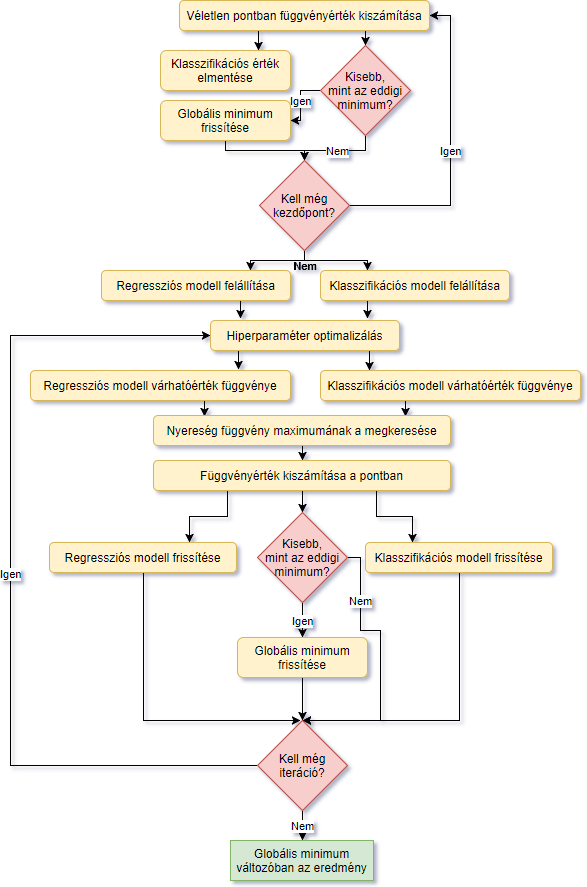
\includegraphics[width=140mm, keepaspectratio]{figures/shogun.png}
	\caption{\texttt{MyShogunOpt.optimize()} algoritmus}
	\label{fig:shogun}
\end{figure}











